\documentclass{article}%
\usepackage[T1]{fontenc}%
\usepackage[utf8]{inputenc}%
\usepackage{lmodern}%
\usepackage{textcomp}%
\usepackage{lastpage}%
\usepackage[head=40pt,margin=0.5in,bottom=0.6in]{geometry}%
\usepackage{graphicx}%
%
\title{\textbf{Teniente Carlos Esqueda llegó a Colombia tras orden de recaptura}}%
\author{ELNACIONAL WEB}%
\date{19/10/2018}%
%
\begin{document}%
\normalsize%
\maketitle%
\textbf{URL: }%
http://www.el{-}nacional.com/noticias/politica/teniente{-}carlos{-}esqueda{-}llego{-}colombia{-}tras{-}orden{-}recaptura\_256477\newline%
%
\textbf{Periodico: }%
EN, %
ID: %
256477, %
Seccion: %
Política\newline%
%
\textbf{Palabras Claves: }%
NO\_TIENE\newline%
%
\textbf{Derecho: }%
1.2%
, Otros Derechos: %
1.10%
, Sub Derechos: %
1.2.2, 1.10.1.1%
\newline%
%
\textbf{EP: }%
NO\newline%
\newline%
%
\textbf{\textit{El militar fue vinculado con el supuesto "Golpe Azul" de 2014 por lo que estuvo cuatro años preso. El pasado jueves fue liberado y a pocas horas después un tribunal dictó orden de recaptura~}}%
\newline%
\newline%
%
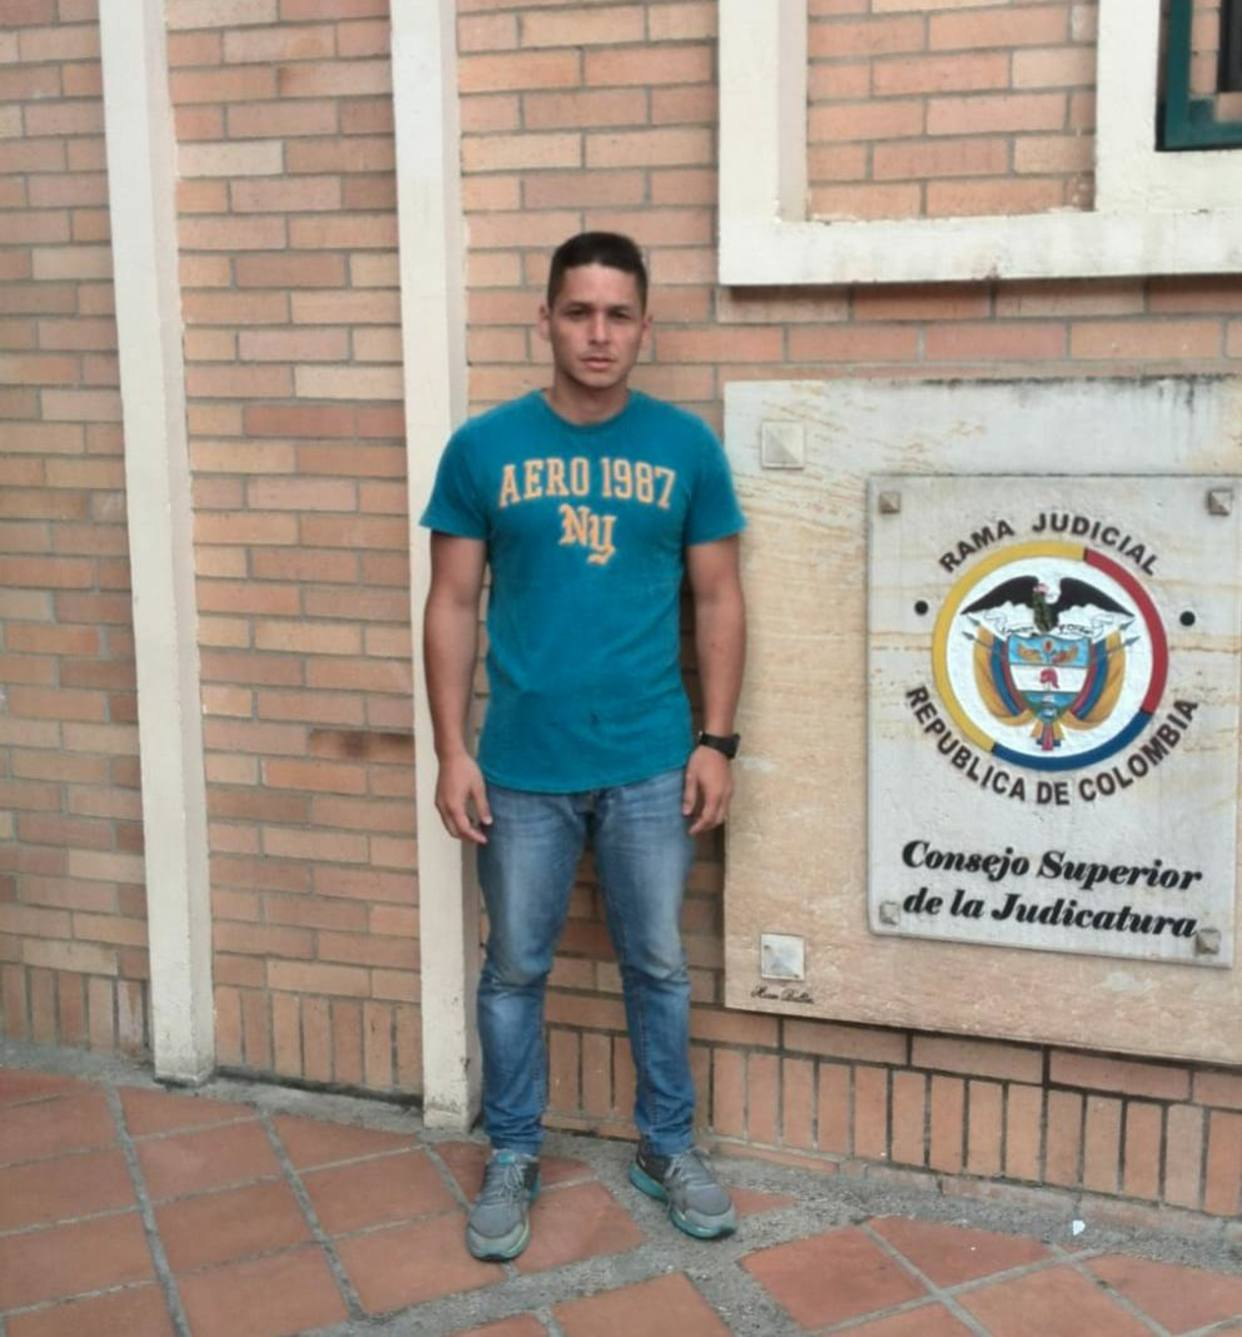
\includegraphics[width=300px]{157.jpg}%
\newline%
%
El primer teniente Carlos José Esqueda Martínez, implicado en el supuesto "Golpe Azul", se encuentra en Colombia luego de que el gobierno venezolano ordenara su recaptura.%
\newline%
%
El militar, al conocer la orden de recaptura, inició su viaje para salir de Venezuela. Una fuente informó este viernes~a~El Nacional Web~que Esqueda se encuentra en Colombia.%
\newline%
%
Esqueda, quien estuvo recluido tres años en la cárcel La Pica,~fue liberado el pasado jueves. A pocas horas de su liberación se dio a conocer la orden de recaptura.%
\newline%
%
\end{document}